% Failure detection of Phase 4. Compile with: pdflatex health_phase4.tex
\documentclass[tikz,border=1pt]{standalone}
\usepackage{mathptmx}
\usetikzlibrary{positioning,arrows.meta,calc}

\begin{document}
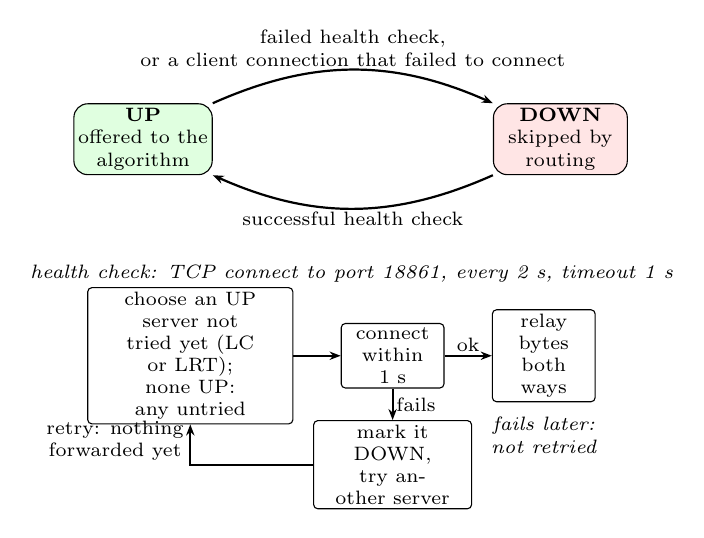
\begin{tikzpicture}[
    >={Stealth[length=4pt,width=3pt]},
    state/.style={draw, rounded corners=5pt, align=center, font=\scriptsize, minimum width=17mm,
                  minimum height=9mm, inner sep=1.5pt},
    stage/.style={draw, rounded corners=1.5pt, align=center, font=\scriptsize, fill=white, inner sep=1.5pt,
                  minimum height=7.5mm},
    lab/.style={font=\scriptsize, align=center, inner sep=1pt},
    note/.style={font=\scriptsize\itshape, align=center, inner sep=1pt},
]
  % ---------------- per-server health state ----------------
  \node[state, fill=green!12] (up) at (0, 0) {\textbf{UP}\\offered to the\\algorithm};
  \node[state, fill=red!10] (down) at (5.3, 0) {\textbf{DOWN}\\skipped by\\routing};
  \draw[->, thick] (up.north east) to[bend left=24]
      node[lab, above] {failed health check,\\or a client connection that failed to connect}
      (down.north west);
  \draw[->, thick] (down.south west) to[bend left=24]
      node[lab, below] {successful health check}
      (up.south east);
  \node[note, anchor=north] at (2.65, -1.55)
      {health check: TCP connect to port 18861, every 2 s, timeout 1 s};

  % ---------------- one client connection ----------------
  \node[stage, text width=25mm] (choose) at (0.6, -2.75) {choose an UP server not\\tried yet (LC or LRT);\\none UP: any untried};
  \node[stage, text width=12mm, right=6mm of choose] (connect) {connect\\within 1 s};
  \node[stage, text width=12mm, right=6mm of connect] (relay) {relay bytes\\both ways};
  \node[stage, text width=19mm, below=4mm of connect] (fail) {mark it DOWN,\\try another server};
  \draw[->, thick] (choose) -- (connect);
  \draw[->, thick] (connect) -- node[lab, above] {ok} (relay);
  \draw[->, thick] (connect) -- node[lab, right] {fails} (fail);
  \draw[->, thick] (fail.west) -| node[lab, pos=0.8, left=1pt] {retry: nothing\\forwarded yet} (choose.south);
  \node[note, anchor=north] at ([yshift=-1.5mm]relay.south) {fails later:\\not retried};
\end{tikzpicture}
\end{document}
